\documentclass[a4paper,11pt,parskip=half]{scrartcl}

%\usepackage[utf8]{inputenc}
\usepackage[T1]{fontenc}
\usepackage{ae}
\usepackage[ngerman]{babel}

\usepackage{graphicx}

\usepackage{color}
\usepackage{listings}

% "define" Scala
\lstdefinelanguage{scala}{
  morekeywords={abstract,case,catch,class,def,%
    do,else,extends,false,final,finally,%
    for,if,implicit,import,match,mixin,%
    new,null,object,override,package,%
    private,protected,requires,return,sealed,%
    super,this,throw,trait,true,try,%
    type,val,var,while,with,yield,%
    imperative,evt},
  otherkeywords={=>,<-,<\%,<:,>:,\#,@},
  sensitive=true,
  morecomment=[l]{//},
  morecomment=[n]{/*}{*/},
  morestring=[b]",
  morestring=[b]',
  morestring=[b]"""
}

\definecolor{dkgreen}{rgb}{0,0.6,0}
\definecolor{gray}{rgb}{0.5,0.5,0.5}
\definecolor{mauve}{rgb}{0.58,0,0.82}

% Default settings for code listings
\lstset{
  frame=tb,
  language=scala,
  aboveskip=3mm,
  belowskip=3mm,
  showstringspaces=false,
  columns=flexible,
  basicstyle={\small\ttfamily},
  numbers=none,
  numberstyle=\tiny\color{gray},
  keywordstyle=\color{blue},
  commentstyle=\color{dkgreen},
  stringstyle=\color{mauve},
  frame=single,
  breaklines=true,
  breakatwhitespace=true
  tabsize=2
}


\begin{document}

\title{ESCALA \\ Convenient Event Expression Language}
\author{David Noack, Michael Tretter}

\maketitle

\section{Einf"uhrung}

ESCALA erweitert Scala um Events, die durch Funktionen ausgel"ost werden k"onnen und auf die wiederum Funktionen reagieren k"onnen.
Allerdings ist die bisher verwendete, nur auf Scala Sprachkonstrukten aufbauende Syntax f"ur Events nicht intuitiv.
Besonders die "Anderung des Eventtypes anhand der "ubergebenen Parameter ist kompliziert.
Daher soll in diesem Praktikum eine neue Syntax entwickelt werden, die die Syntax f"ur Events vereinfacht, mehr an das "ubliche Bild von Scala anpasst und es erlaubt Eventparameter mit dem Namen zu referenzieren.

Als Beispiel nehmen wir folgendes imperative Event, das ein Int als ersten und ein String als zweiten Parameter enth"alt:
\begin{lstlisting}
imperative evt e[Int,String]
\end{lstlisting}

Wir m"ochten nun ein zweites Event darauf reagieren lassen, bei dem jedoch die Parameter vertauscht sind. 
In alter Syntax muss mit einer map-Funktion das Event zum neuen Typ transformiert werden.
Im Code sieht das folgenderma{\ss}en aus:
\begin{lstlisting}
evt e_old[String,Int] = e.map((n: Int, s: String) => (s,n))
\end{lstlisting}

Die neue Syntax verzichtet auf die map-Funktion und erreicht die Definition des neu definierten Events durch namentliche Bindung der funktionalen Parameter an die tats"achlichen Parameter des gebundenen Events.
Die Schreibweise weist gro{\ss}e "Ahnlichkeit zu den Parametern beim Pattern Matching auf und sollte daher intuitiv zu verwenden sein.
\begin{lstlisting}
evt e_new(s: String,n: Int) = e(n, s) // Vertauschen von Parametern
evt e1(n: Int) = e_new(_, n) // Weglassen eines Parameters
evt e2(n: Int) = e_new(_, n) || e1(n) // Verodern zweier Events
\end{lstlisting}

Dieses Praktikum implementiert die neue Syntax im dem Umfang, dass einfache Events aneinander gebunden oder verodert werden k"onnen und die Parameter direkt gebunden, vertauscht oder weggelassen werden k"onnen.
Die daf"ur notwendigen Schritte f"ur die jeweiligen Phasen des Compilers werden im Folgenden detailliert vorgestellt.

\section{Parser}

Der Parser akzeptiert sowohl neue Syntax mit Parameterlisten als auch alte Syntax.
Allerdings lassen sich beide Syntax nicht mischen, daher sind in neuer Syntax nur Konstrukte m"oglich, die bereits implementiert sind.

\paragraph{Linke Seite}
Der Parser erkennt neue Syntax anhand einer sich hinter dem Identifier "offnenden runden Klammer.
Er parst dann den kompletten Ausdruck als neue Syntax.
F"ur die Parameterliste greift der Parser auf eine Funktion, die auch beim Parsen der Parameterlisten von Funktionen und Case-Klassen verwendet wird, zur"uck.
Diese war zuvor lokal und ist nun global aufrufbar.
Ist die Parameterliste leer, wird sp"ater Unit als Parametertyp erzeugt.

\paragraph{Rechte Seite}
Die rechte Seite (\emph{rhs}) wird wie in alter Syntax als simple expression geparst.
Die Unterscheidung der rhs findet erst im Typer statt.

\paragraph{AST-Knoten}
Der Ergebnisknoten des Parser im abstrakten Syntaxbaum (\emph{AST}) ist ein EventDef statt einem ValDef, um im AST zwischen alter und neuer Syntax unterscheiden zu k"onnen.
Die EventDef verwendet eine List[ValDef] statt einem Tree, um die Parameter zu speichern.
So ist es m"oglich, statt nur der Typen, die Typen und Parameternamen mit zu "ubergeben.
\begin{lstlisting}
def EventDef(
  tree: Tree, 
  mods: Modifiers, 
  name: Name, 
  vparams: List[ValDef], 
  rhs: Tree)
\end{lstlisting}

Anhand der EventDef ist es m"oglich Events im Typer gesondert zu behandeln.

\section{Namer}

Im Namer werden die Informationen zu einer EventDef-Knoten erweitert und im Kontext aktualisiert.
Das bedeutet zu einer EventDef werden ein Getter erzeugt, die Flags erweitert und ein entsprechendes Symbole erzeugt und in den Scope eingef"ugt.

Die Methode \texttt{eventSig} erzeugt Symbole f"ur alle Parameter, ermittelt die Typen der Parameter und setzt den Typ des Events auf die Eventklasse aus der Bibliothek anhand der ermittelten Typen.
Eine leere Parameterliste erzeugt den EventTyp Unit.
Ein einzelner Parameter erzeugt als EventTyp den Typen dieses Parameters.
Mehrere Parameter werden als Tupel an den EventTyp gebunden.

Da Events maximal eine Parameterliste mit sich f"uhren, musste die Methode \texttt{enterValueParam} aus \texttt{enterValueParams} extrahiert werden.
Diese Methode aktualisiert die Informationen zu einem Parameter, erzeugt ein Symbol und "ubergibt diese Information an die EventDef.

\section{Typer}

Der Typer transformiert eine EventDef in eine ValDef.
Das bedeutet, dass nach dem Typer neue Syntax und alte Syntax identisch sind und keine gesonderte Weiterbehandlung n"otig ist.

Im ersten Schritt wird der EventTyp anhand der Parameterliste nach dem gleichen Schema wie im Namer erzeugt.

% todo unterscheidung der Events????
\paragraph{Transformation des Event durch Mapping}
Die alte Syntax verwendet eine map-Funktion, um Events unterschiedlicher Typen aneinander zu binden.
Dieses Verhalten wird in diesem Schritt nachgebildet.
Kernschritt der Transformation ist daher die Erzeugung eines map-Knotens, der eine Funktion auf das gebundene Event anwendet. 
Diese Funktion bildet die Parameter des gebundenen Events auf die Parameter des definierten Events ab.
Die Erstellung dieser Funktion wird im n"achsten Paragraph beschrieben.

Zur Optimierung werden die Typen und Parameternamen des definierten und des gebundenen Events verglichen, bevor das Mapping durchgeführt wird.
Wenn diese in Typ und Reihenfolge der Parameternamen "ubereinstimmen, wird auf das Mapping verzichtet und die Events ohne Transformation verbunden.

Eine Sonderbehandlung erfahren rhs, die Wildcards enthalten.
Eine solche rhs erh"alt im AST nicht einen Apply-Knoten, der im Typer erwartet wird, sondern einen Function-Knoten, der neue ValDefs f"ur die Wildcards als Parameter besitzt.
Dieser Fall wird behandelt, indem die Parameter des Function-Knoten zu den Eventparametern hinzugef"ugt werden und die Transformation danach auf das eigentliche Event anwendet wird.

Folgendes Listing zeigt die Transformation des einfachen Beispiels als Code:
\begin{lstlisting}
e_new(s: String, n: Int) = e(n, s) // vor der Transformation
e_new = e.map((n: Int, s: String)=>(s, n)) // nach der Transformation
\end{lstlisting}

Abbildung \ref{fig:ast} zeigt die Transformation des Beispiels im AST.
\begin{figure}[h]
  \centering
  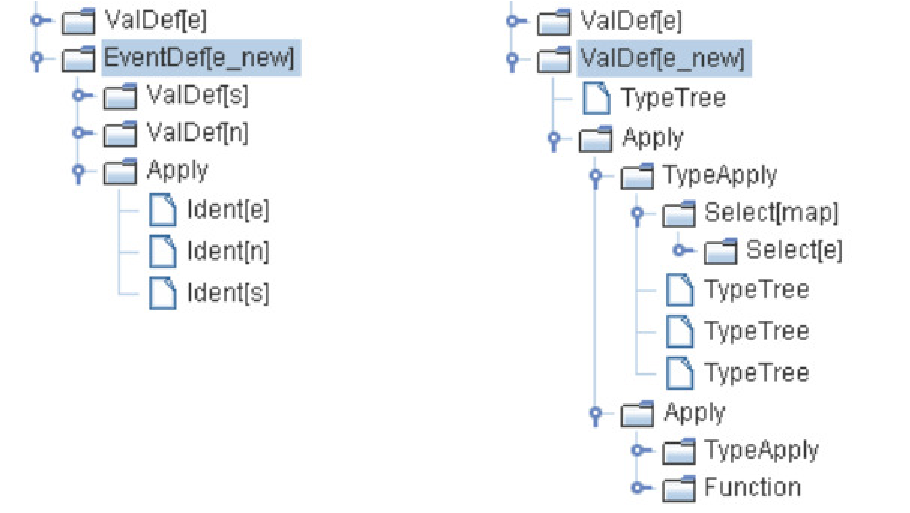
\includegraphics[width=.6\linewidth]{ast}
  \caption{Der AST des Beispiels vor (links) und nach (rechts) dem Typer}
  \label{fig:ast}
\end{figure}

\paragraph{Erzeugung der Transformationsfunktion}
Die Funktion, die an den map-Knoten gebunden wird, wird erzeugt indem eine Parameterliste und ein Ergebnistupel einzeln erzeugt und aneinander gebunden werden.
Die Parameterliste enth"alt die neuen Parameternamen mit Typen in der Reihenfolge des gebundenen Events.
Das Ergebnistupel legt die Reihenfolge der Parameter f"ur das definierte Event fest.
Die Parameterliste wird erzeugt, indem f"ur jeden tats"achlichen Parameter des gebundenen Events ein neuer ValDef-Knoten erzeugt wird, der die Eigenschaften des gleichnamigen funktionalen Parameters des definierten Events besitzt.
Es werden Ident Knoten mit den Namen der funktionalen Parameter erzeugt, um die tats"achlichen Parameter in der Reihenfolge der funktionalen Parameter zu referenzieren. 
Anschlie{\ss}end werden sie zum Ergebnistupel zusammengefasst.
Parameterliste und Ergebnistupel werden in einem Function-Knoten verbunden und an den map-Knoten gebunden.

Durch diese Transformation entsteht Unabh"angigkeit vom genauen Aufbau des gebundenen Events und die Umformung funktioniert auch f"ur alle Ausdr"ucke die ein Event vom richtigen Typ als R"uckgabewert haben.

\paragraph{Or-Events}
Ein Or-Event kann anhand der Veroderungsfunktion (||) gefunden werden.
Dieses Event wird in die Teilevents zerlegt, die beide einzeln mit map zum definierten Event transformiert werden.
Anschlie{\ss}end werden die Events wieder durch die vorhandenen Mechanismen verkn"upft.

\paragraph{Fehlerbehandlung}
Auf folgende Fehler wird explizit gepr"uft:
\begin{itemize}
  \item Der R"uckgabewert der rechten Seite ist kein Event.
  \item Eine Name, der in der rechten Seite verwendet wird, wurde nicht im Event deklariert.
\end{itemize}
Folgende Fehler werden implizit gepr"uft:
\begin{itemize}
  \item Ein Parameter des definierten Events wird nicht auf der rechten Seite verwendet.
  \item Der Typ des definierten Event entspricht nicht der Transformation des gebundenen Events.
\end{itemize}

% W"urde ich ganz weglassen
%\section{Erg"anzungen von Lucas}

%\begin{itemize}
%\item Parameterbehandlung
%\item Setzen der korrekten Symbol im Namer
%\item Getter f"ur der Event im Namer in das symbol eingef"ugt
%\end{itemize}

\section{M"ogliche Erweiterungen}
In Zukunft sollten alle anderen m"oglichen Eventtransformationen aus der alten Syntax in die neue Syntax aufgenommen werden.
Dazu z"ahlen in erster Linie Und-Events (auch im Hinblick auf Eventintervalle) und die M"oglichkeit explizit Werte an Parameter zu binden.

\end{document}
